
\section{Motivation and Problem Formulation}\label{sec:motivation}

\subsection{Storage Minimization and Proposed Concept of Distributed Channel Storage}

\begin{figure}[t]
{\figurefontsize
\centering
\input{Fig/device_storage.pdf_tex}
\caption{Storage mechanisms. (a) Storage with dedicated unit. (b) \textcolor{red}{Channel
storage.} (c) Port of dedicated storage unit.}
\label{fig:device_storage}
}
%\vspace{-0.5cm}
\end{figure}

The sequencing graph of an assay defines the dependency of operations. These
operations are scheduled to devices in a given order for execution. Different
schedules, however, yield different storage usage and transportation
requirements.
%
In \figname~\ref{fig:pcr}(b) and \ref{fig:pcr}(c), two schedules
for the PCR assay are shown, where one mixer is used to execute the
operations. The first schedule executes the operations in the order
$o_1\to o_2\to o_3 \to o_4 \to o_6 \to o_5\to o_7$. After executing $o_1$, the
intermediate result should be transported to the storage unit, so that the device
can be reused to execute $o_2$. When $o_6$ is executed, it takes the result of
$o_4$ from the mixer directly as one input and fetches the result of $o_3$
from the storage unit. In this schedule, in total four storage operations
and four fetch operations are needed. In addition, the results of $o_1$,
$o_2$ and $o_3$ stay in the storage unit at the same time, so that the
capacity requirement of the storage unit is three.
In the schedule in \figname~\ref{fig:pcr}(c) with the execution order
$o_1\to o_2\to o_5 \to o_3 \to o_4 \to o_6\to o_7$,
however, there are only three store and three fetch operations,
leading to a storage capacity of only two units.
In addition, the execution
time of the assay in the second schedule is even shorter.

The comparison of the two schedules in \figname~\ref{fig:pcr}(b) and
\ref{fig:pcr}(c) demonstrates that the schedule scheme affects the
transportation of fluid samples as well as the required capacity of the storage unit,
and the execution time of the assay may be unnecessarily prolonged if storage
and transportation are not considered properly.
This important problem, however, has not been dealt with by previous
methods.



\begin{comment}
\begin{figure}[t]
    \centering
	 \subfloat[]{
       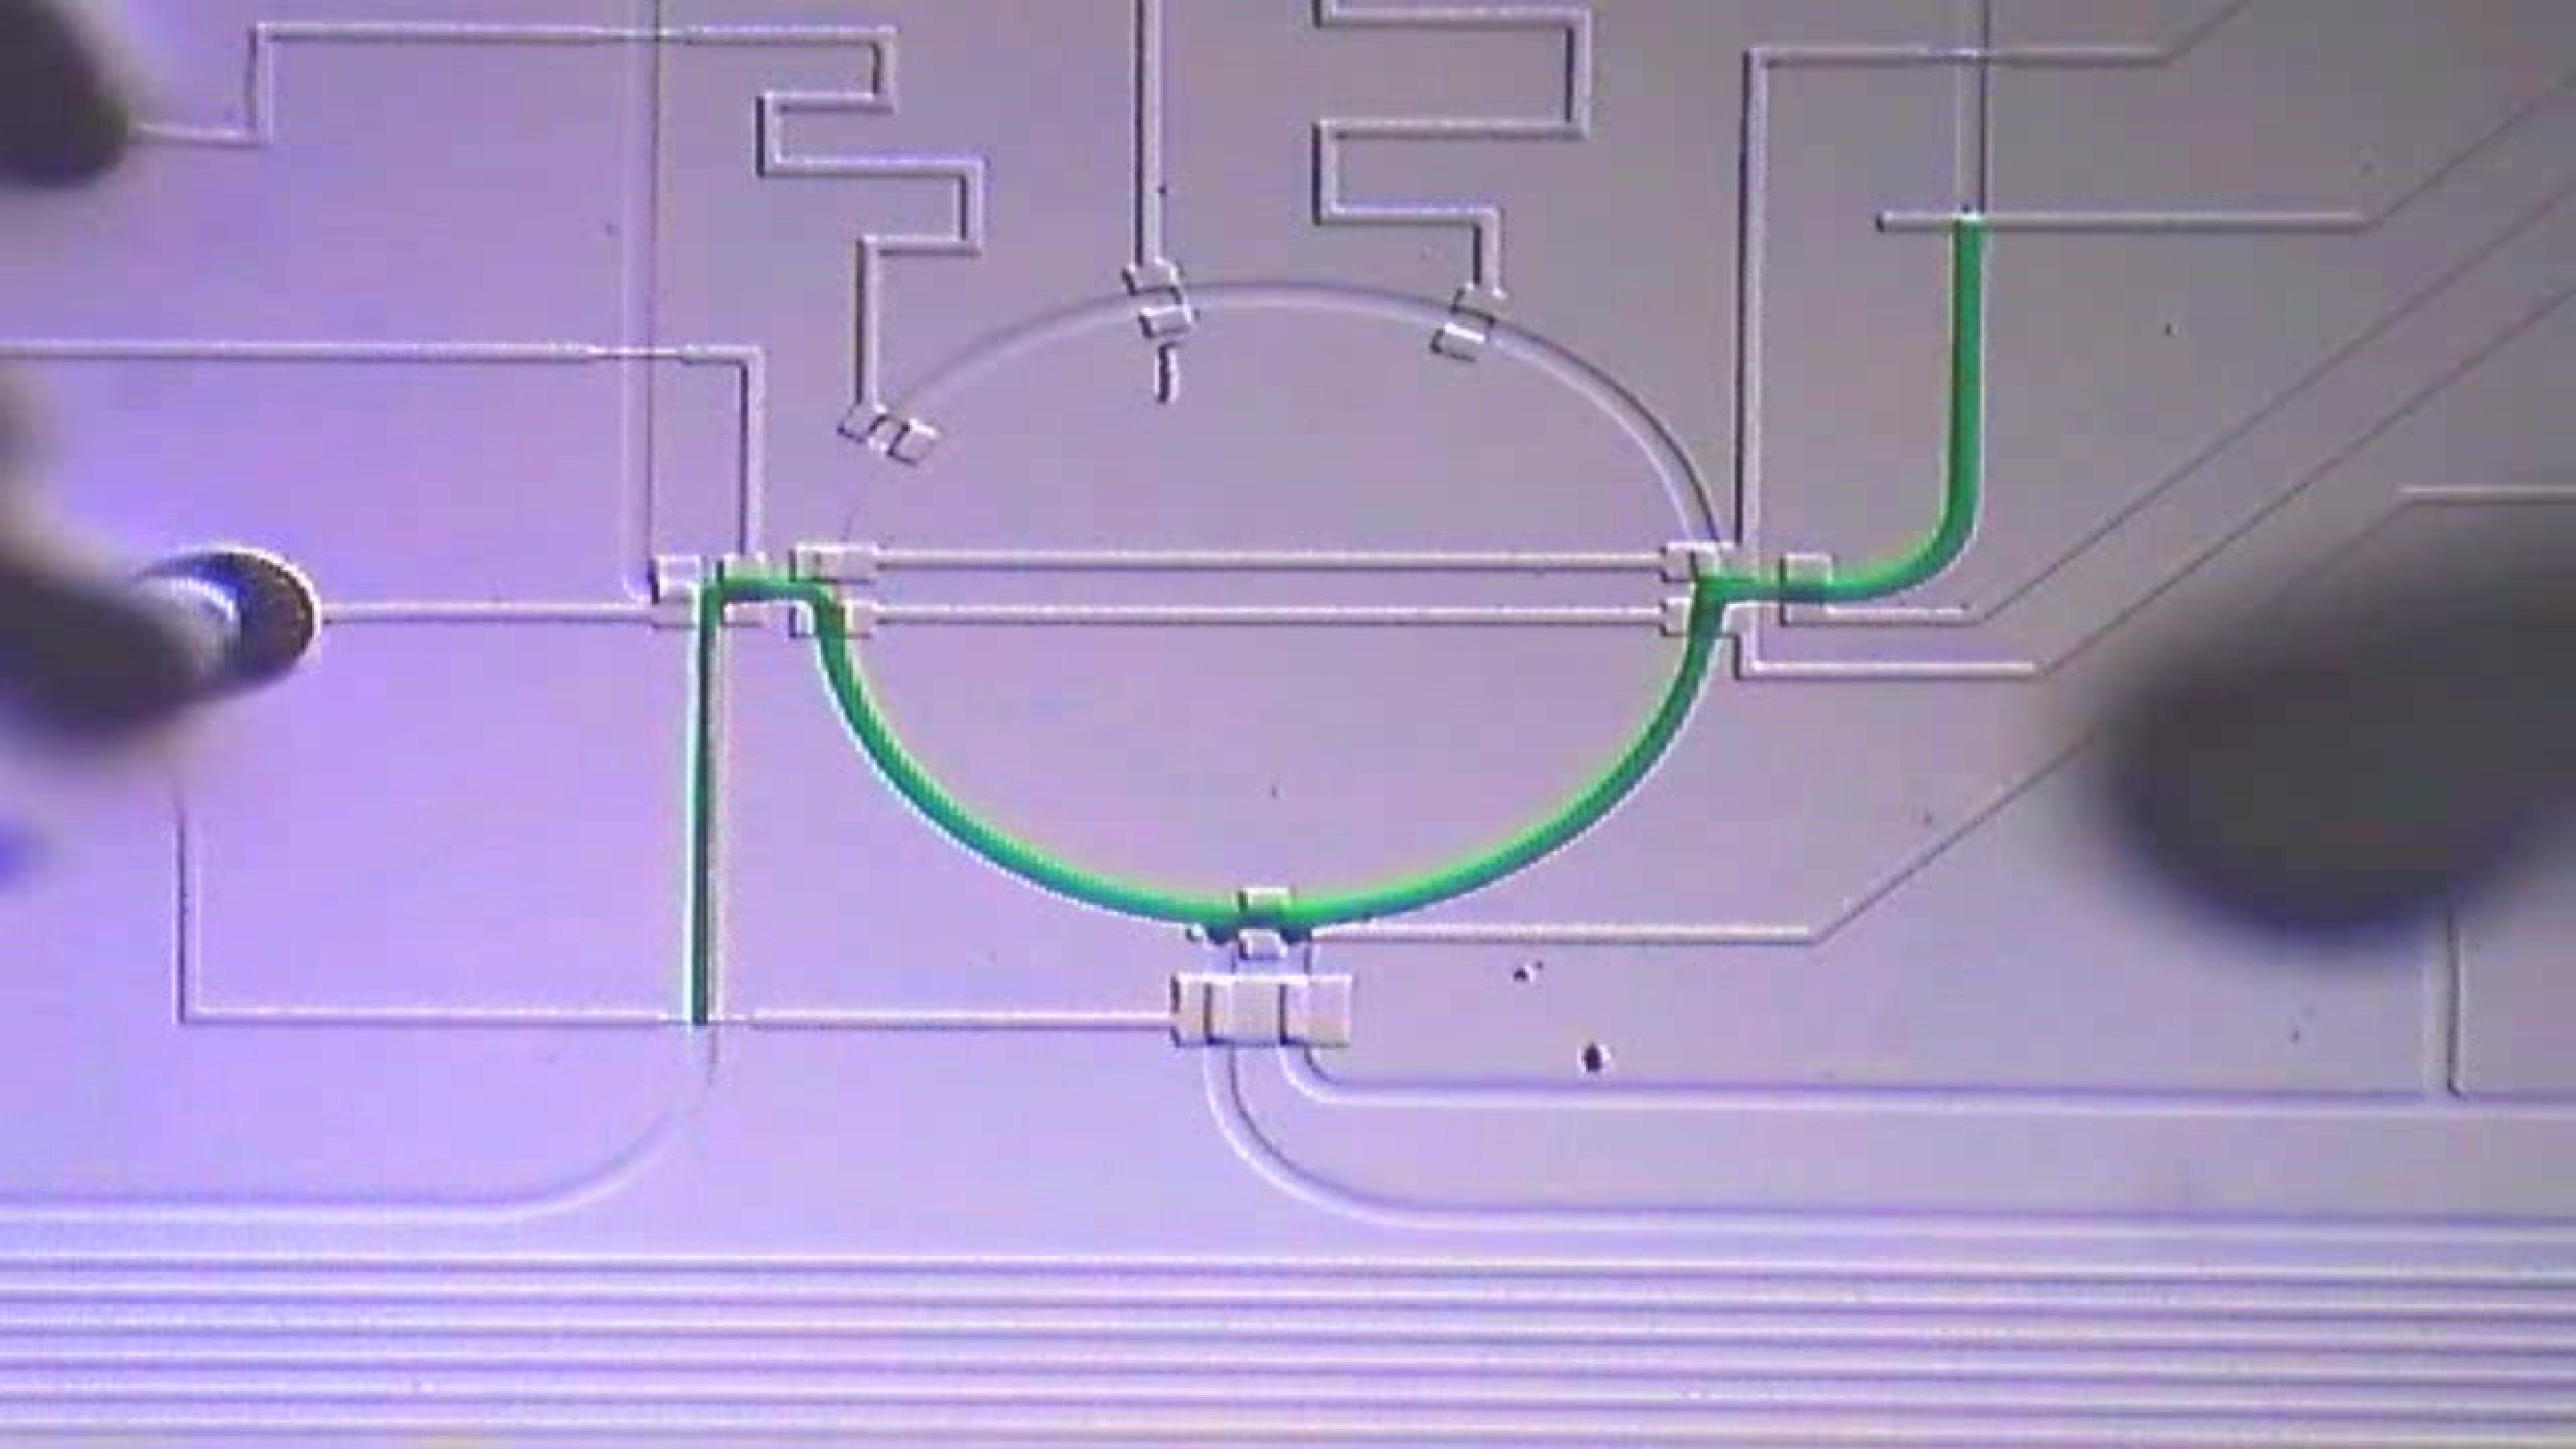
\includegraphics[width=0.45\linewidth]{Visio/mix1.pdf}}
	 \subfloat[]{
        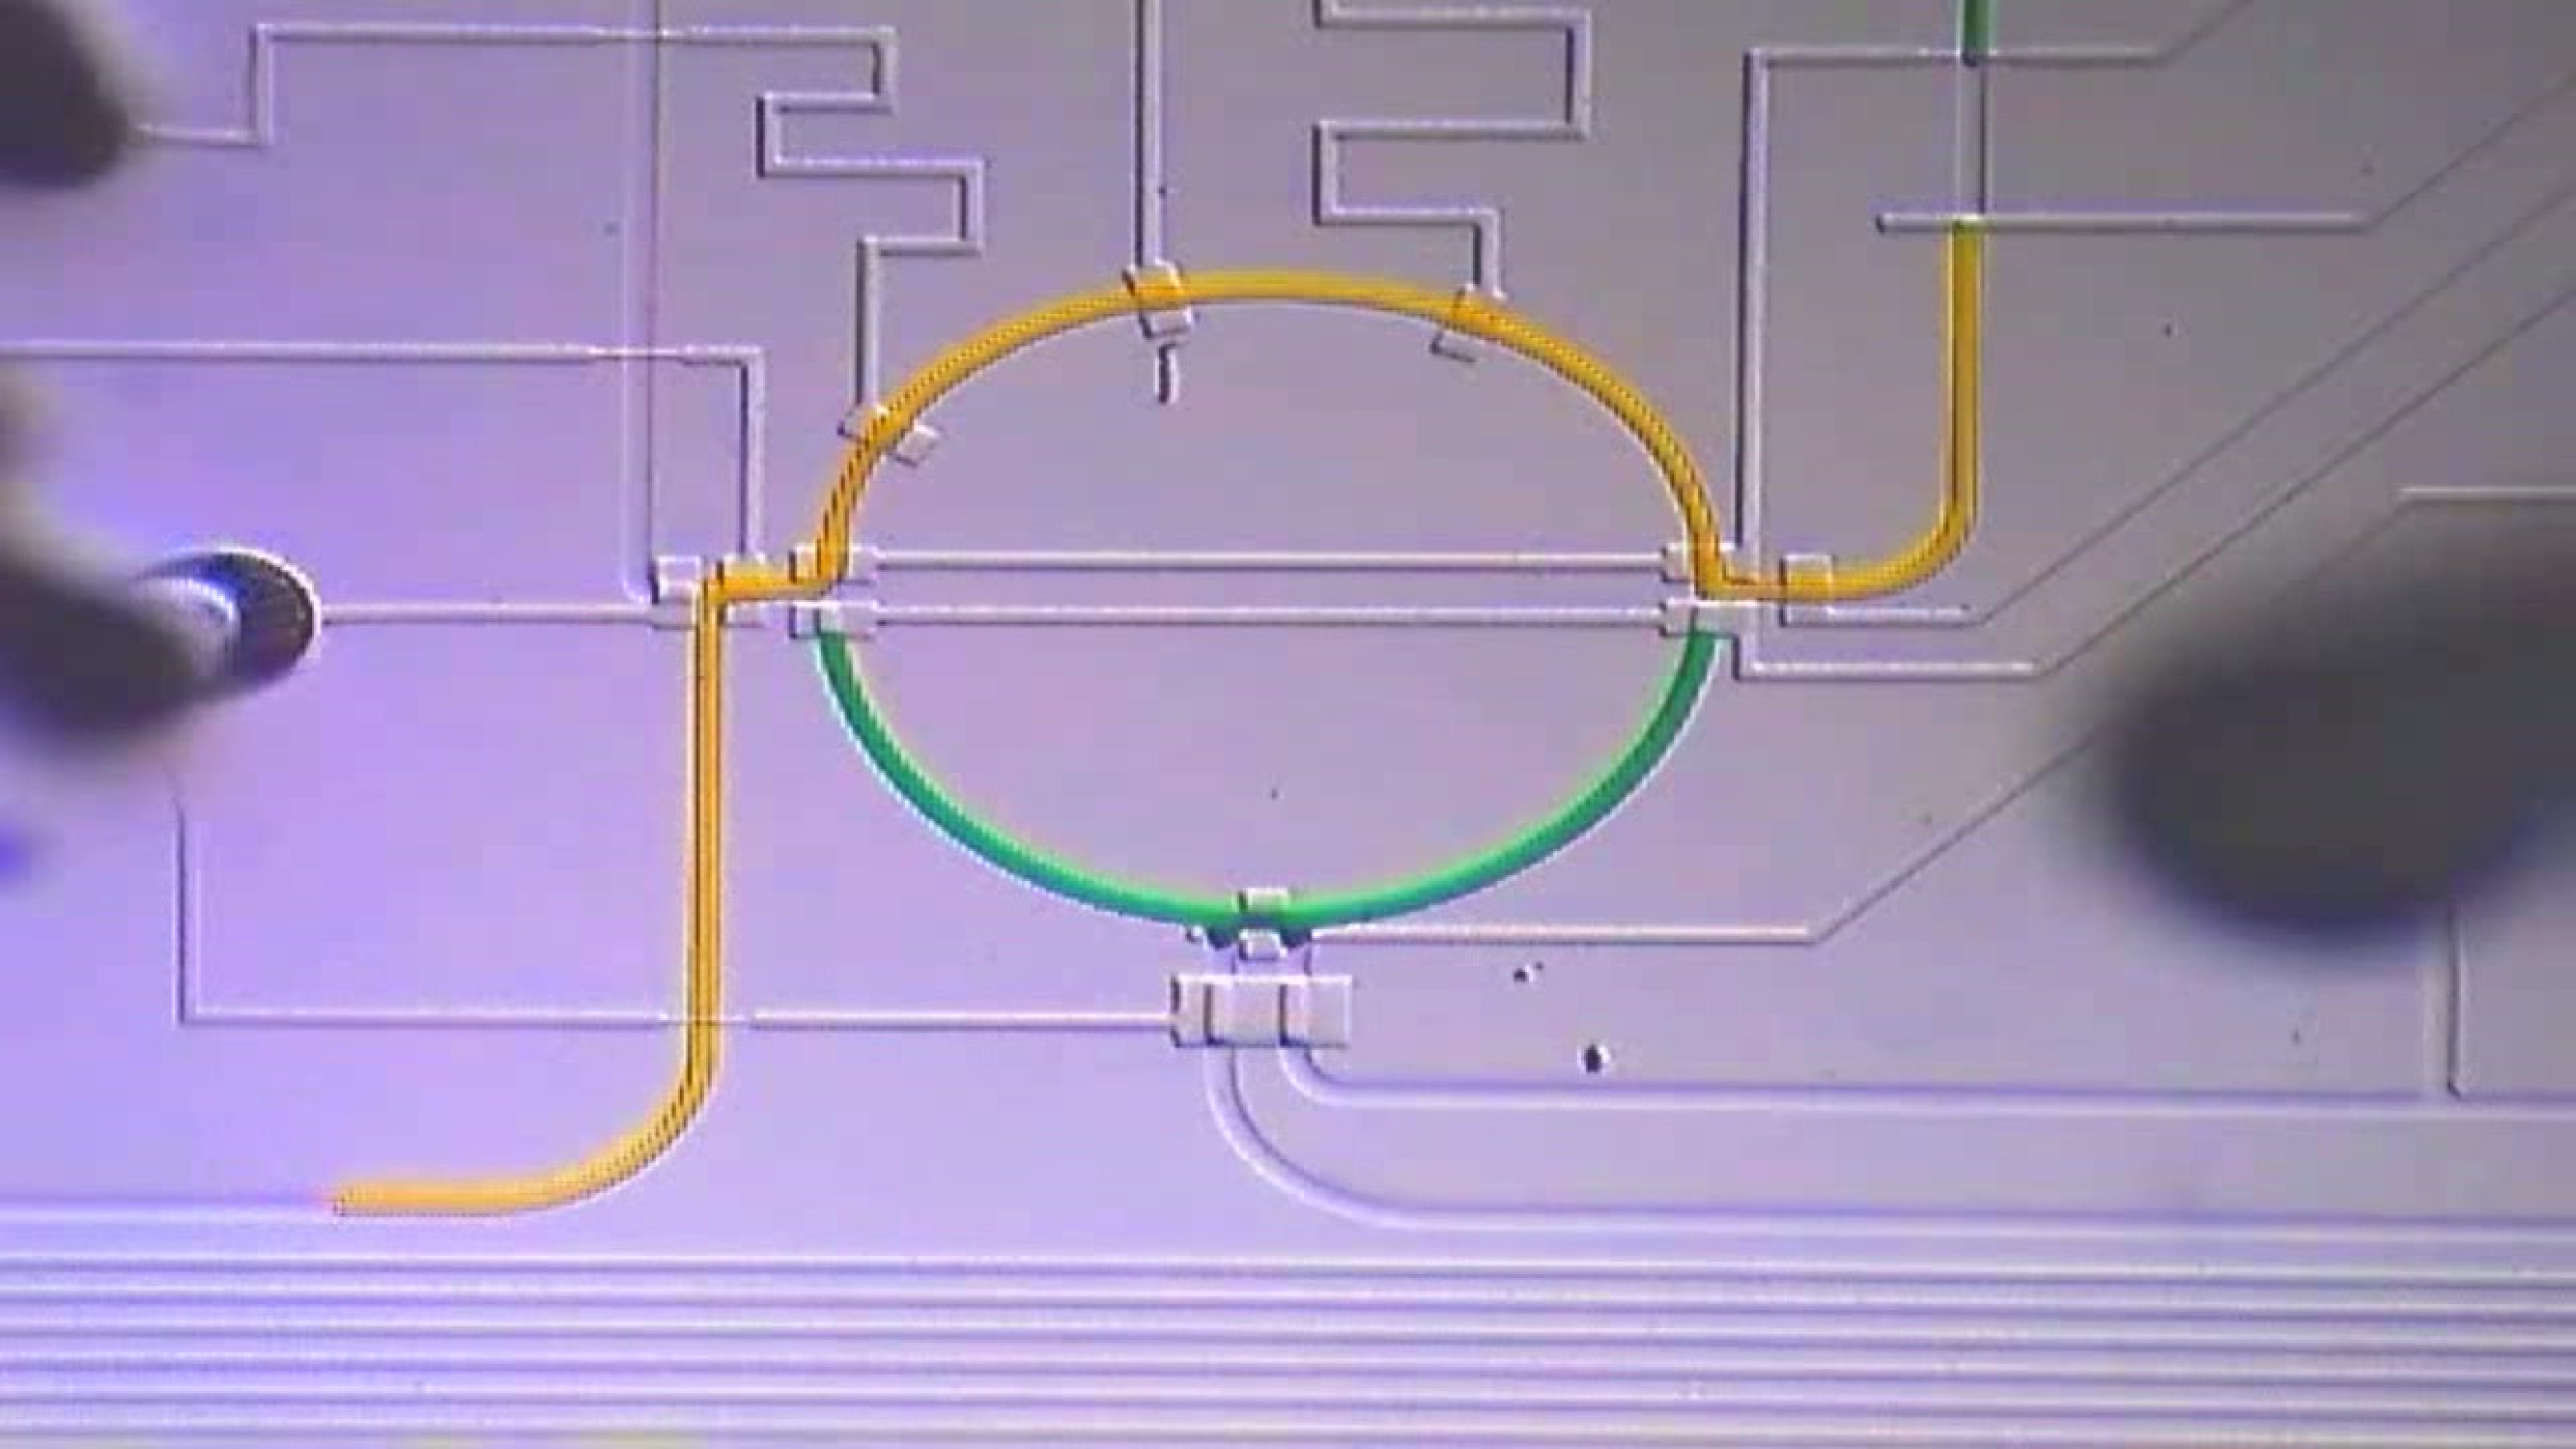
\includegraphics[width=0.45\linewidth]{Visio/mix2.pdf}}
     \\
     \subfloat[]{
        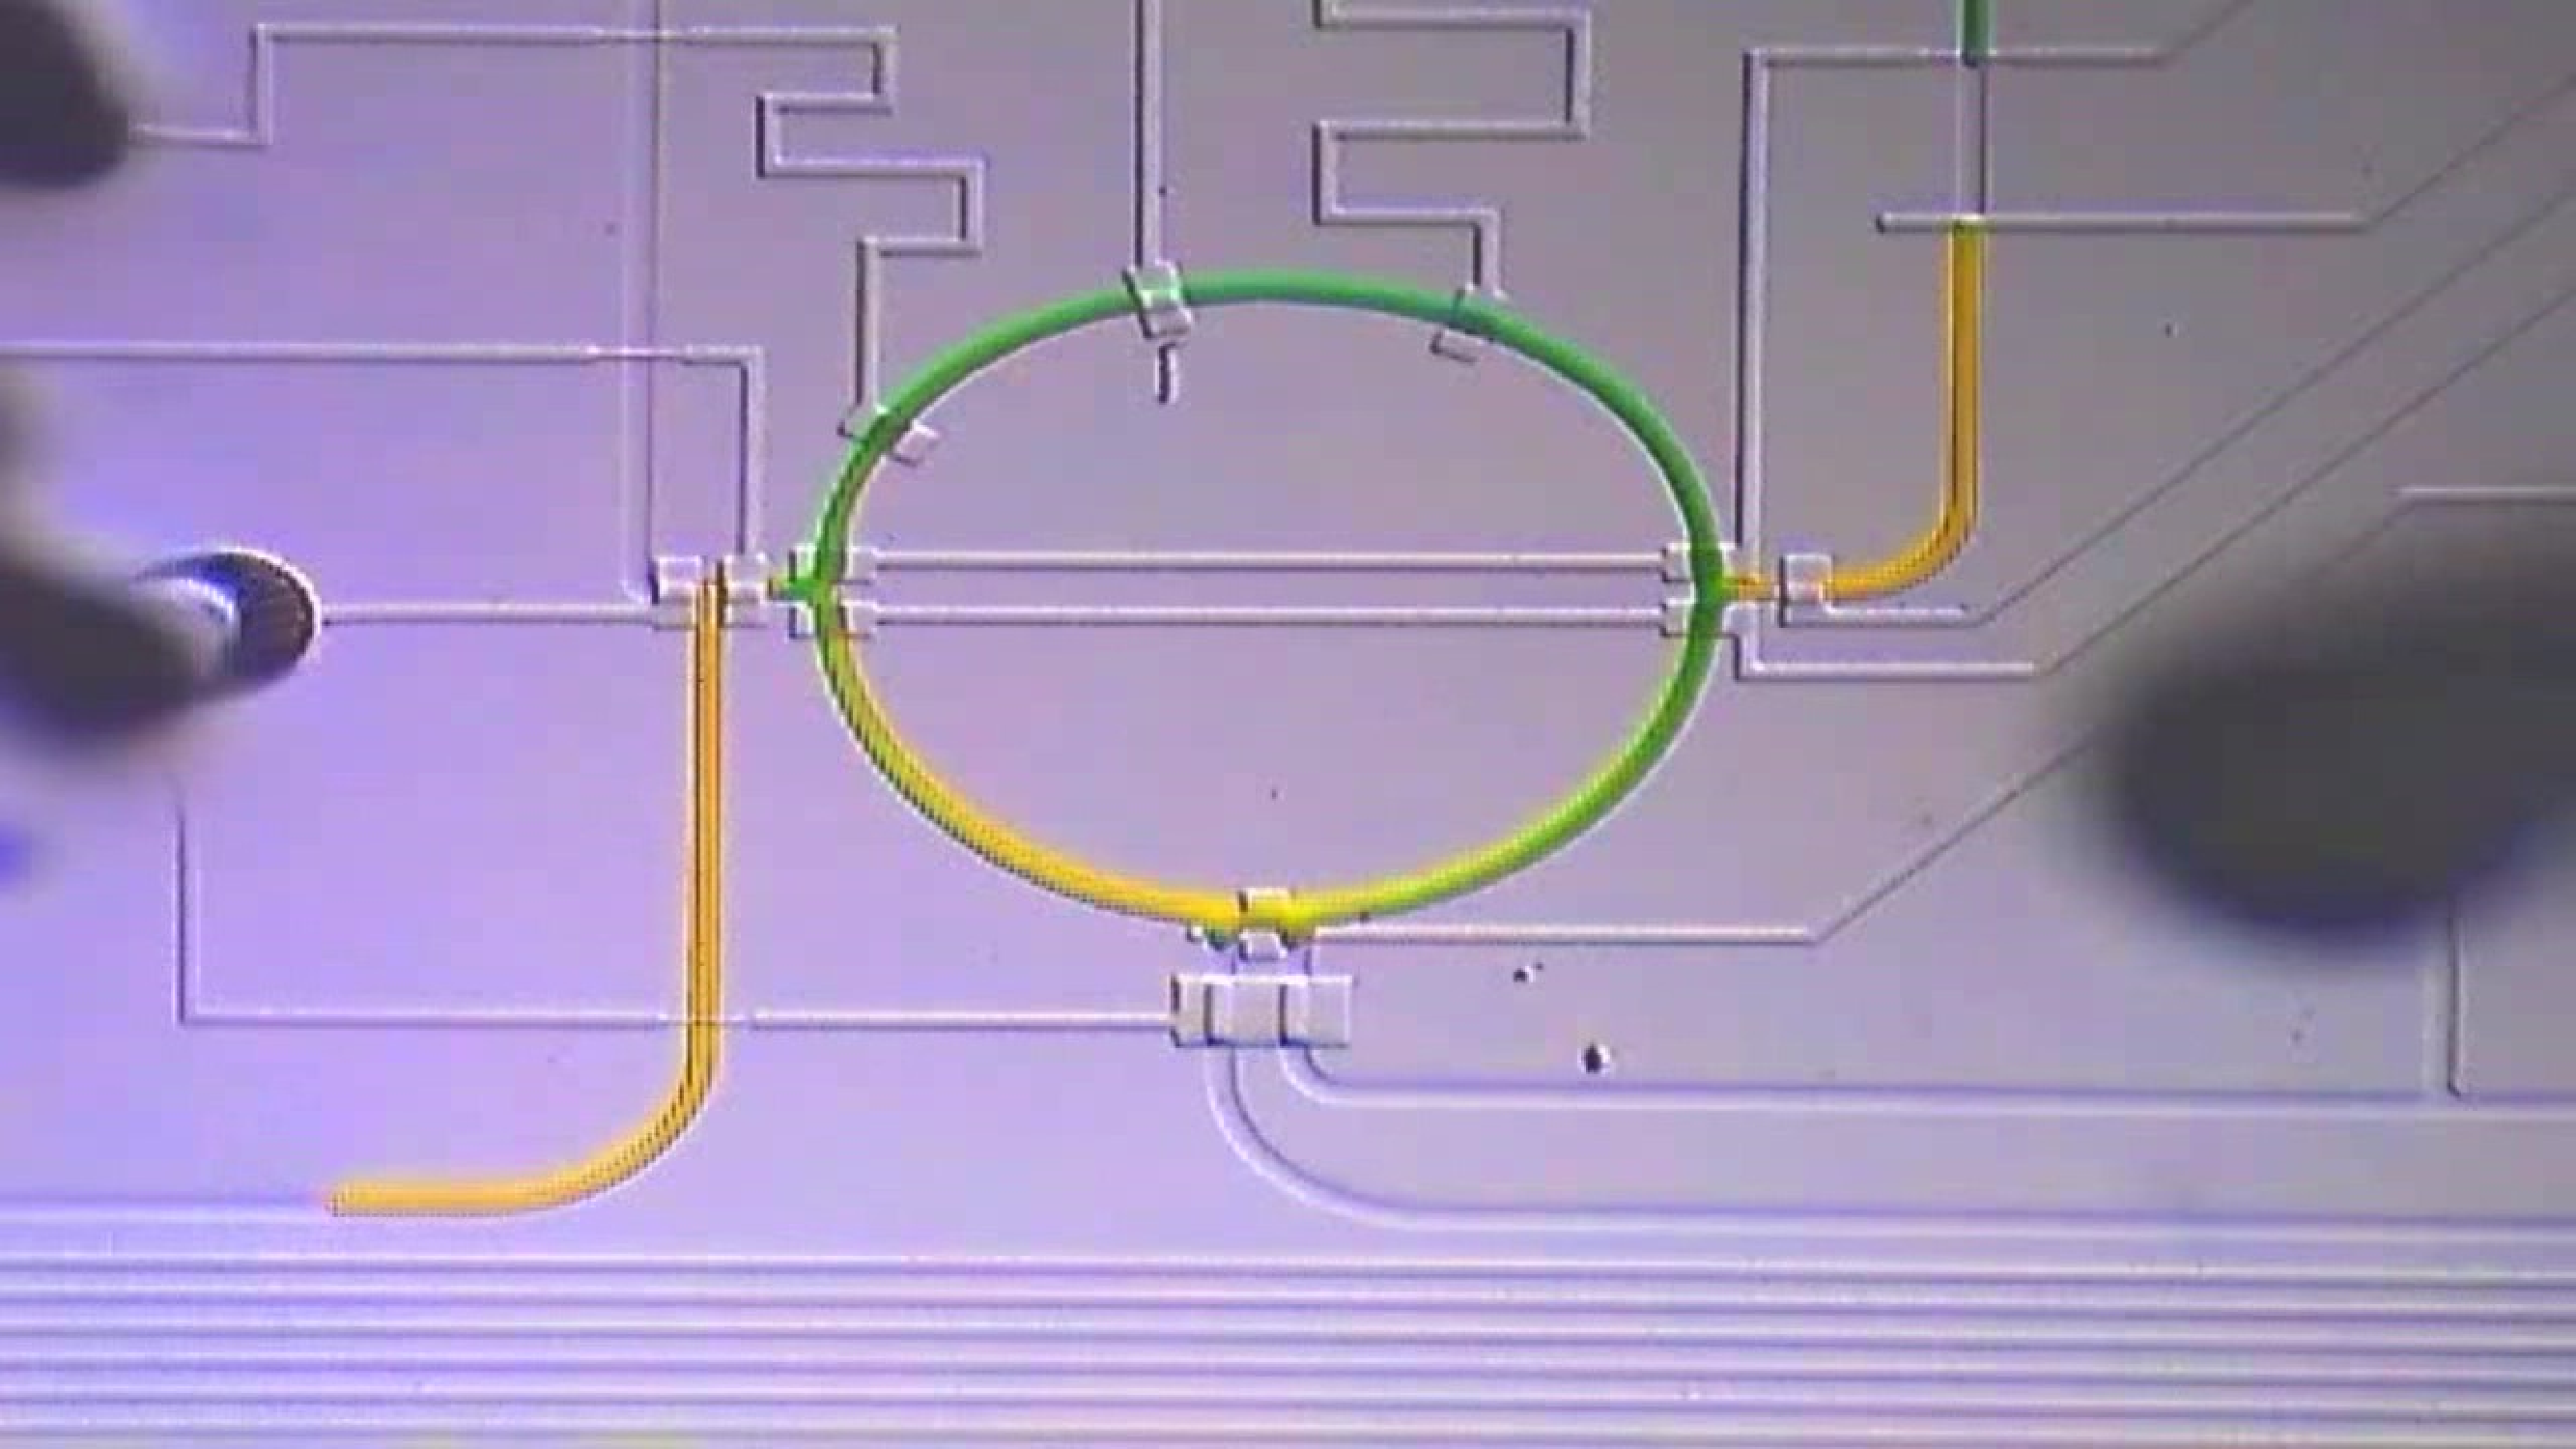
\includegraphics[width=0.45\linewidth]{Visio/mix3.pdf}}	
     \subfloat[]{
        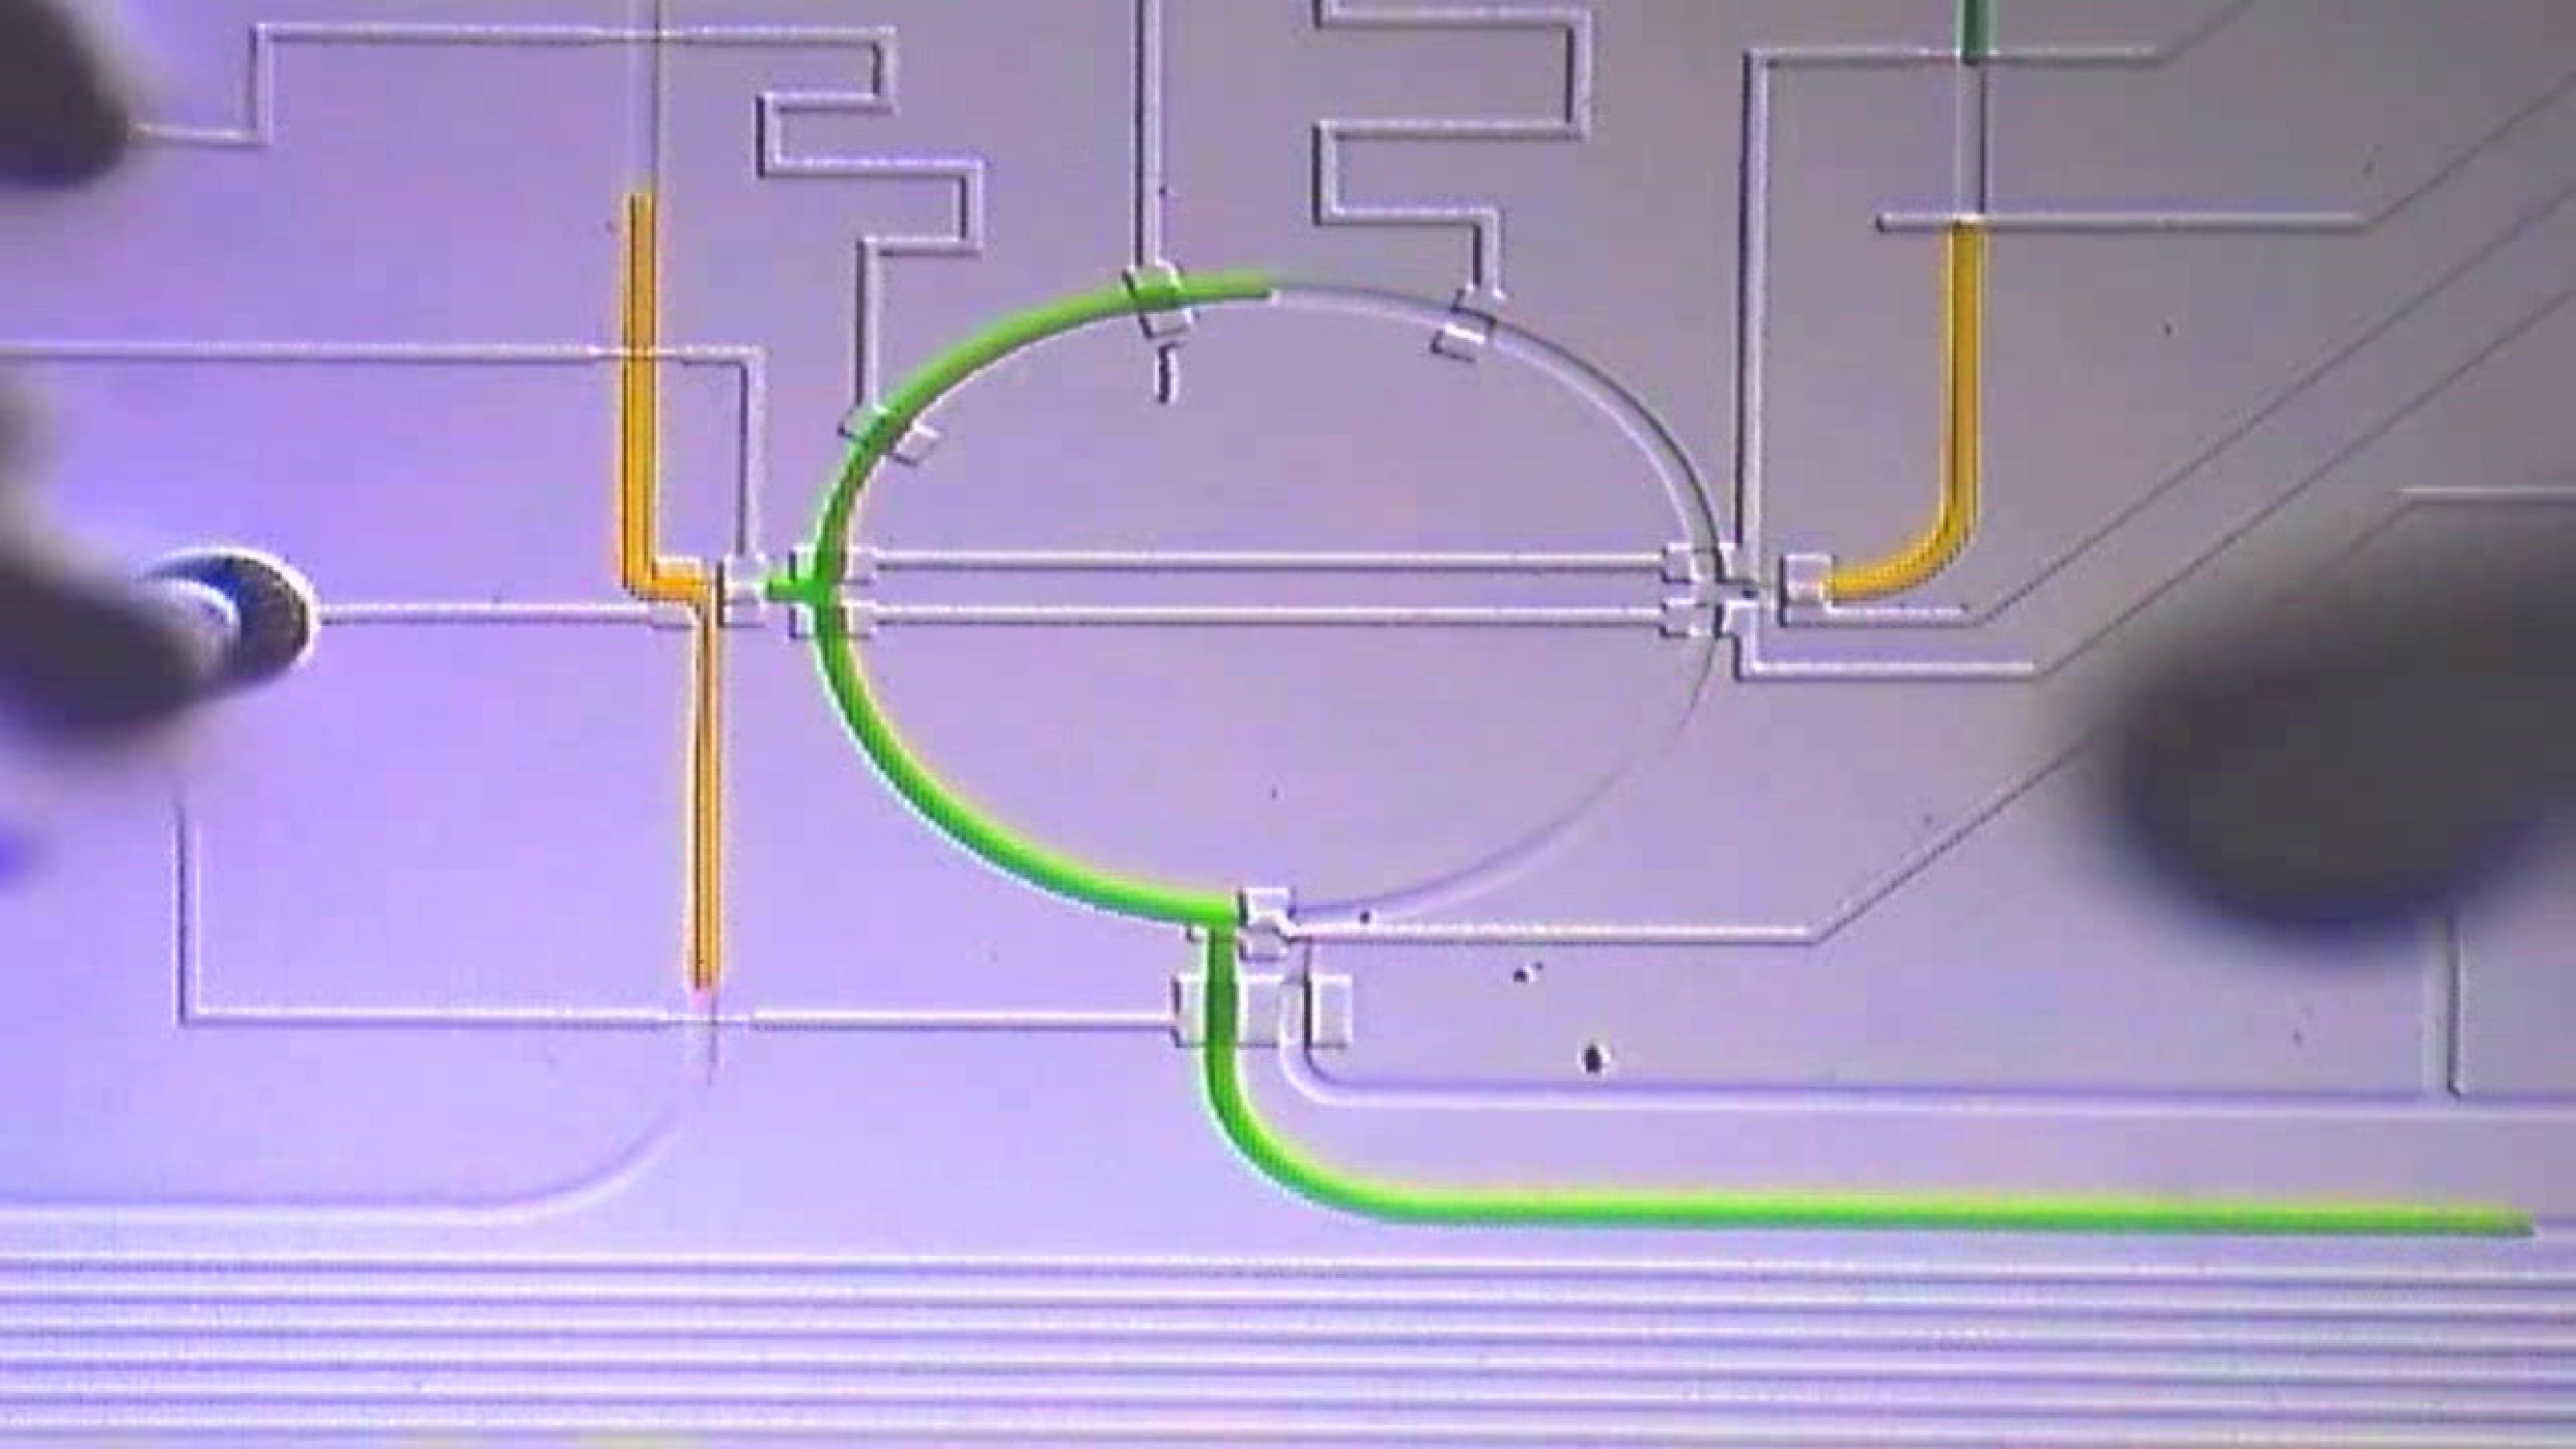
\includegraphics[width=0.45\linewidth]{Visio/mix4.pdf}}
	  \caption{Snapshots of fluid caching when performing the mixing operation using a flow-based microfluidic biochip \cite{mixing}. (a) Step 1: loading the first fluid flow into the lower half of the mixer, (b) step 2: loading the second fluid flow into the upper half of the mixer, (c) step 3: sealing the mixer and starting the mixing operation, and (d) step 4: removing the mixture and excess fluids.}
	  \label{fig:mixing}
\vspace{-0.5cm}
\end{figure}
\end{comment}



When a fluid sample is stored, it is transported to the storage unit through a
channel. The diagram of a simple chip with one mixer and one storage unit is
shown in \figname~\ref{fig:device_storage}(a). When this chip is used to execute
the operation $o_1\to o_2\to o_5$ in the schedule in
\figname~\ref{fig:pcr}(c), the mixer first stores the result of $o_1$ in the
storage unit. After $o_2$ is finished, the result of $o_1$ is fetched back to
the mixer to execute the operation $o_5$.
In this case,  the channel itself instead of a dedicated
storage unit is sufficient to store the intermediate result from $o_1$,
as shown in \figname~\ref{fig:device_storage}(b). \textcolor{red}{Note that valves need to be placed at the two ends of the channel, so that the fluid can be cached in the channel safely.} This example demonstrates that
fluid samples can in fact be cached  within temporary
storage constructed from channel segments. This distributed storage can also
overcome the bandwidth limit problem at the ports of the dedicated storage unit
illustrated in \figname~\ref{fig:valve_mixer_storage}(c)
and \figname~\ref{fig:device_storage}(c), where multiple fluid samples must be queued when they access the storage unit
simultaneously.

\begin{figure}[t]
    \centering
	 \subfloat[]{
       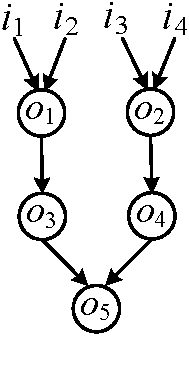
\includegraphics[width=0.16\linewidth]{Visio/sequencing_graph.pdf}}
    \label{ta}
	\subfloat[]{
        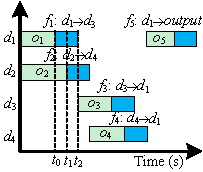
\includegraphics[width=0.42\linewidth]{Visio/scheduling.pdf}}
    \label{tb}
    \subfloat[]{
        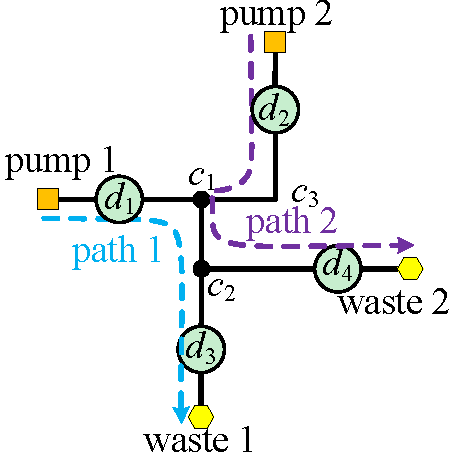
\includegraphics[width=0.35\linewidth]{Visio/chip_architecture.pdf}}
    \label{tc}
	  \caption{Flow-path planning. (a) Sequencing graph of a bioassay. (b) A scheduling and binding solution with minimized execution time. (c) Flow paths constructed on a given chip architecture.}
	  \label{fig:motivation}
\vspace{-0.5cm}
\end{figure}

\subsection{Design Challenges in Flow-Path Planning}\label{sec:flow_path_chan}

\begin{figure*}[t]
    \centering
	 \subfloat[]{
       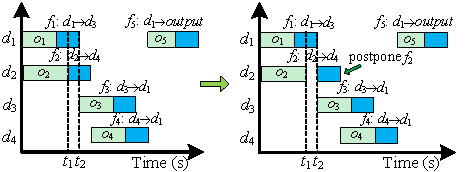
\includegraphics[width=0.55\linewidth]{Visio/scheduling_adjustment.pdf}}
    \label{ta1}
	\subfloat[]{
        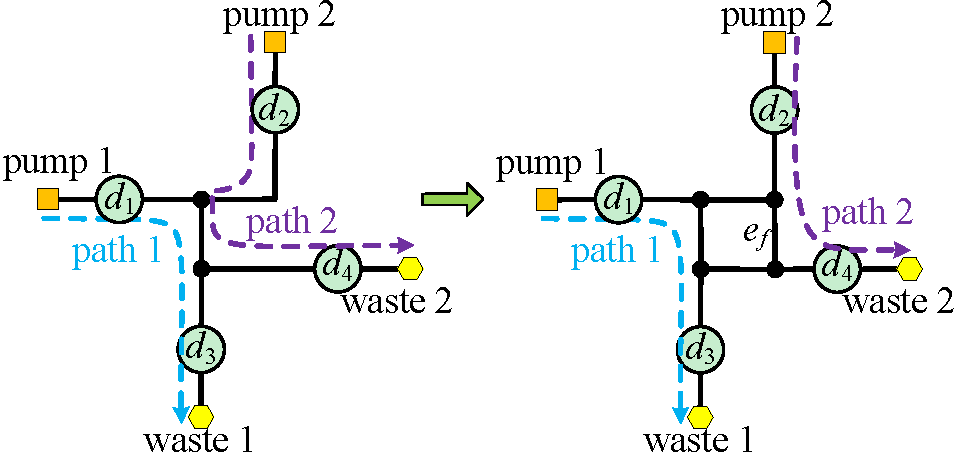
\includegraphics[width=0.43\linewidth]{Visio/new_path.pdf}}
    \label{tb1}
	  \caption{Strategies for transportation conflict elimination. (a) Scheduling adjustment. (b) Architecture ajustment.}
	  \label{fig:strategy}
%\vspace{-0.5cm}
\end{figure*}

When executing bioassays on a microfluidic biochip, fluid samples need to be transported to specific devices/channel segments at certain time windows according to the scheduling and binding solution and this, undoubtedly, requires a carefully planned flow-channel network to complete these tasks. For a  transportation task between two devices denoted as $d_i$ and $d_j$, to drive the movement of fluid, an external pressure source or a mechanical pump needs to be connected to $d_i$ to produce thrust. Moreover, to avoid channel blockage after the completion of the corresponding operation, waste liquid that is not needed anymore should be discarded, thus requiring a waste port connected to $d_j$. As a consequence, the pump, the two devices, the waste port, as well as the channel segments connecting them form the complete flow path of the transportation task.

We take the sequencing graph shown in Fig.~\ref{fig:motivation}(a) as an example to illustrate the flow-path planning on a certain biochip. Fig.~\ref{fig:motivation}(b) shows a scheduling and binding solution with minimized execution time of the bioassay described in Fig.~\ref{fig:motivation}(a), where four devices ($d_1$--$d_4$) are allocated and five transportation tasks ($f_1$--$f_5$) are scheduled to execute corresponding operations. For example, in task $f_1$, the resulting fluid of operation $o_1$ is required to be transported to device $d_3$ as an input sample of operation $o_3$, leading to a flow path from $d_1$ to $d_3$. Fig.~\ref{fig:motivation}(c) shows a given biochip architecture, on which $path\;1$ is a feasible flow path starting with a mechanical pump, passing through devices $d_1$ and $d_3$, and ending at a waste port. Note that a valid flow path should bypass those devices  occupied by other on-going operations as well as flow channels used for fluid caching.



\subsubsection{Transportation conflict}

Since several transportation tasks may be performed concurrently in a scheduling scheme,
to avoid potential transportation conflicts, flow paths among these tasks need to be considered systematically. Let us revisit the scheduling scheme in Fig.~\ref{fig:motivation}(b). Since the time windows for executing transportation tasks $f_1$ and $f_2$ overlap with each other, the corresponding flow paths cannot share any on-chip resource, including pump ports, channel segments, etc. For example, $path\;1$ and $path\;2$ in Fig.~\ref{fig:motivation}(c) are flow paths constructed for tasks $f_1$ and $f_2$, respectively. These two paths, however, are essentially in transportation conflict with each other, since switches $c_1$ and $c_2$ as well as the channel segment between them are shared by both paths. Worse still, we cannot even find a valid path-planning solution for the two tasks due to the limited on-chip resources in Fig.~\ref{fig:motivation}(c).

Accordingly, we propose two conflict elimination techniques, \textsl{scheduling adjustment} and \textsl{architecture adjustment} as illustrated in Fig.~\ref{fig:strategy}, to fundamentally solve the transportation conflict discussed above. %Note that when two fluidic flows pass through the same channel segment one after the other, the second flow can be contaminated by the residue left behind by the first flow, resulting in a cross-contamination between them. This problem can be solved by injecting a buffer fluid into the chip to wash the corresponding channels \cite{hu2015wash}.


\begin{easylist}
&\textit{Scheduling adjustment}: The goal of scheduling adjustment is to eliminate transportation conflicts in a flow-path planning solution by postponing the execution of some transportation tasks. As illustrated in Fig.~\ref{fig:strategy}(a), to eliminate the conflict between the flow paths described in Fig.~\ref{fig:motivation}(c), the execution of transportation task $f_2$ is postponed by the scheduling adjustment operation, so that tasks $f_1$ and $f_2$ do not overlap in their execution time. As a result, the shared channel segment between switches $c_1$ and $c_2$ in Fig.~\ref{fig:motivation}(c) can be used by both paths sequentially, although the completion time of the bioassay is increased slightly.

&\textit{Architecture adjustment}: Another strategy to eliminate the transportation conflicts is to introduce extra resources to the biochip architecture directly, so that the previously shared on-chip resources can be released from conflicts. For example, in Fig.~\ref{fig:strategy}(b), a channel segment $e_f$ with two extra switches is added to the chip architecture, leading to a new flow path for transportation task $f_2$. Since the new path does not share any resource with that of task $f_1$, the previous conflict is removed from the chip successfully.

\end{easylist}

\subsubsection{Caching deadlock}

\begin{figure}[t]
    \centering
	 \subfloat[]{
       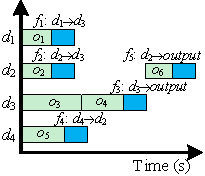
\includegraphics[width=0.5\linewidth]{Visio/caching_deadlock1.pdf}}
    \label{ta}
	\subfloat[]{
        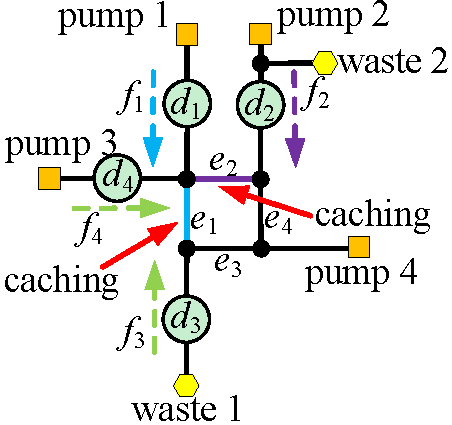
\includegraphics[width=0.44\linewidth]{Visio/caching_deadlock2.pdf}}
    \label{tb}
	  \caption{Illustration of caching deadlock. (a) Scheduling scheme of a bioassay. (b) A flow-path planning solution with caching deadlock.}
	  \label{fig:deadlock}
%\vspace{-0.5cm}
\end{figure}

Another issue that needs to be considered during flow-path planning is caching deadlock. Since flow channels in a distributed channel-storage architecture fulfill the dual functions of transportation and caching, channel segments used for fluid caching may block the normal transportation of other fluids, thereby leading a deadlock of the flow-channel network. For example, when mapping the scheduling scheme described in Fig.~\ref{fig:deadlock}(a) to the biochip architecture shown in Fig.~\ref{fig:deadlock}(b), the resulting fluids of operations $o_1$ and $o_2$ need to be transported from devices $d_1$ and $d_2$ to $d_3$, respectively. To wait for the completion of operation $o_3$, whose resulting fluid is another input of operation $o_4$, the two fluids are temporally cached in channel segments $e_1$ and $e_2$, thus blocking the flow path of transportation task $f_4$. To solve this problem, one feasible solution is to desynchronize the execution of these transportation tasks by employing an idea similar to the proposed scheduling adjustment strategy. For example, if the execution of $f_4$ is postponed to a point in time that the fluid cached in either $e_1$ or $e_2$ has been removed, the deadlock in Fig.~\ref{fig:deadlock}(b) can be eliminated. Another way to solve this problem is to release these blocked channels by directly moving the corresponding cached fluids to other unused channel segments. For example, if the resulting fluid of $o_2$ is moved to either channel segment $e_3$ or $e_4$ for caching, the deadlock can also be eliminated.



\subsection{Problem Formulation}

Based on the proposed concept of distributed channel storage, the synthesis problem considering architecture design and path planning in flow-based microfluidic biochips can be formulated as follows:

\begin{easylist}
&\textit{Inputs}: The sequencing graph of a biochemical assay;
the execution durations of all operations; the maximum numbers of devices allowed
in the chip.

&\textit{Outputs}: A schedule minimizing intermediate fluid storage; a channel
caching schedule including the locations and the time slots
of fluid samples stored temporarily in channels; a biochip architecture with the exact flow paths to manipulate the transportation/caching of fluid samples without conflict.

&\textit{Objectives}: Minimizing the overall resource usage and the completion time of the bioassay.
\end{easylist}


